\documentclass[11pt]{article}

% ---- Page geometry ----
\usepackage[letterpaper, margin=1in]{geometry}

% ---- Typography ----
\usepackage[T1]{fontenc}
\usepackage{microtype}

% ---- Math ----
\usepackage{amsmath}
\usepackage{amssymb}

% ---- Tables ----
\usepackage{booktabs}
\usepackage{array}
\usepackage{multirow}

% ---- Figures ----
\usepackage{graphicx}
\usepackage{caption}
\usepackage{subcaption}
\usepackage{float}

% ---- Colors and links ----
\usepackage{xcolor}
\usepackage[colorlinks=true, linkcolor=blue!60!black, citecolor=green!50!black, urlcolor=blue!70!black]{hyperref}

% ---- References ----
\usepackage[numbers,sort&compress]{natbib}
\bibliographystyle{unsrtnat}

% ---- Algorithm ----
\usepackage[ruled,vlined,linesnumbered]{algorithm2e}

% ---- TikZ ----
\usepackage{tikz}
\usetikzlibrary{positioning, arrows.meta, calc, fit, backgrounds}

% ---- Misc ----
\usepackage{enumitem}
\usepackage{adjustbox}
\usepackage[normalem]{ulem} % for \sout in evidence hierarchy

% ---- Custom commands ----
\newcommand{\feat}[1]{\texttt{#1}}
\newcommand{\rtalign}{\feat{r2a\_alignment}}

% ============================================================
\title{Behavioral Exhaust Mining: What Internal Reasoning Structure\\Reveals About Agent Task Success}
\author{Anonymous}
\date{}

\begin{document}
\maketitle

% ============================================================
\begin{abstract}
We study whether structural properties of agent reasoning traces are associated with task success in code repair.
Across 373 validated runs (183 Claude Sonnet~4.6, 190 Codex GPT-5.4) on 75 SWE-bench Lite tasks, we extract 24 primary behavioral features (plus 3 supplementary) from reasoning text and tool-call sequences at zero API cost.
We find that behavioral structure---not linguistic hedging---carries signal: academic hedge vocabulary \citep{hyland2005metadiscourse} shows no association with outcomes in either model ($\rho \approx 0$, $p = 0.60$), while structural features like maximum error streak and early error rate are significantly associated with failure in both models within the same repository.
Linguistic features are model-specific: contrastive marker density shows a confirmed polarity flip, positively associated with success in Sonnet ($\rho = +0.282$, $p = 0.008$) but negatively in Codex ($\rho = -0.264$, $p = 0.020$) on matched tasks.

We discover a thinking/message polarity reversal: tentative language in internal reasoning blocks is significantly associated with failure (permutation $p = 0.0012$), while expressed correction in agent messages is associated with success---the two layers carry structurally different information.
A Sonnet-specific interaction between deliberation length and diagnostic precision yields 73\% pass rate ($n = 22$), exceeding either feature alone (23--38\%).
All behavioral signals degrade over the trajectory: early and mid-stage features discriminate pass from fail, but late-stage features do not.
A leave-one-task-out cross-validation with nested feature selection confirms out-of-sample signal for structural features (Codex AUC = 0.634, permutation $p < 0.001$; Sonnet AUC = 0.569, $p = 0.064$).

These findings establish that agent behavioral exhaust carries model-specific signal associated with task success, motivating intervention testing in future work.
Our initial initial lead finding---reasoning-to-action alignment---was retracted after within-repo permutation testing revealed between-repository confounding ($p = 0.35$), demonstrating the necessity of the confound-control methodology we introduce.
\end{abstract}

% ============================================================
\section{Introduction}
\label{sec:intro}

Autonomous coding agents now routinely solve software engineering tasks that, until recently, required human developers.
On benchmarks like SWE-bench Lite \citep{jimenez2024swebench}, frontier models resolve 40--50\% of real-world bug reports with no human intervention.
Yet deploying these agents outside controlled benchmarks demands something benchmarks do not measure: knowing \emph{when not to trust the agent's output}.
A human developer who watches an agent edit the wrong file, chase a red herring for twenty minutes, or silently break an unrelated test needs a signal---ideally before the damage is done---that the current trajectory is going wrong.

The standard tools for estimating model reliability are largely unavailable in agentic settings.
Log-probabilities, which underpin calibration in classification tasks, are not exposed by most agent-serving APIs.
Sampling-based approaches like self-consistency require multiple completions of long, expensive trajectories.
And the multi-turn structure of agent interaction---where each tool call conditions on the results of previous calls---means that a confidence estimate at step~$t$ must account for the accumulated state of steps~1 through~$t{-}1$, a problem that single-turn calibration methods were not designed to address.

Three families of approaches have emerged.
The first elicits confidence scores directly from the model, either through verbalized probability estimates or softmax-derived scores; this is unreliable for agents because self-reported confidence is poorly calibrated when the model's context accumulates errors over a multi-turn trajectory \citep{kadavath2022language,xiong2024can,xuan2026confidence}.
The second deploys external critics---a second model, a formal verifier, or a human reviewer---to evaluate the agent's actions; this works but scales poorly, as every gated decision requires an additional inference call \citep{cuadron2025shepherd}.
The third, and least explored, asks whether the behavioral exhaust that agents already produce---reasoning text, tool-call sequences, error patterns---contains extractable signal about task success.
This signal is zero-cost (the exhaust already exists in the trace), non-invasive (no prompt modification required), and adds no latency to the agent's execution.

This paper investigates the third approach.
We extract 24 primary behavioral features from agent reasoning traces across 373 validated runs on 75 SWE-bench Lite tasks, using only regex and string matching---no additional model calls.
The features span three tiers: structural properties of the tool-call sequence (error streaks, edit timing), linguistic properties of reasoning text (deliberation length, contrastive markers), and domain-specific properties that bridge reasoning and action (diagnostic precision, file-reference density in thinking blocks).
All runs are independently validated by replaying agent edits on fresh environments and running the target test suite; agent self-report is never used for labeling.

Our central finding is that \textbf{behavioral structure, not linguistic hedging, is associated with task success}.
Academic hedging vocabulary---the ``perhaps,'' ``might,'' ``possibly'' words that are informative in question-answering reasoning chains \citep{vanhoyweghen2025lexical}---carries zero signal in coding agent traces ($\rho \approx 0$, $p = 0.60$).
What does carry signal is how the agent \emph{structures} its reasoning: how long it deliberates per action, how early it encounters errors, and whether its internal thinking contains precise references to the code artifacts it will modify.

These associations are model-specific.
Across the two models in our study, only structural features (consecutive error streaks, early error rate) transfer.
Every linguistic feature that survives rigorous testing is specific to one model, and one feature---contrastive marker density---shows a confirmed polarity flip: it is positively associated with success in Sonnet ($\rho = +0.282$, $p = 0.008$) but negatively associated with success in Codex ($\rho = -0.264$, $p = 0.020$), within the same repository and task set.

The signal also degrades over the trajectory.
In the early and middle thirds, behavioral features discriminate pass from fail; in the final third, they do not ($\rho \approx 0$, $p > 0.6$).
This has a direct implication for gating: behavioral gates should focus on early and mid-trajectory decisions, where the signal is strongest.

We report five contributions:

\begin{enumerate}[leftmargin=*]
\item \textbf{Trajectory-dependent signal quality in agent behavioral features.}
All behavioral features degrade over the agent's trajectory: early and mid-stage features discriminate pass from fail ($p < 0.03$), but late-stage features carry no signal ($\rho \approx 0$, $p > 0.6$).
This suggests that behavioral monitoring, if viable, should focus on early trajectory, when the signal-to-noise ratio is highest.

\item \textbf{A cross-model comparison revealing model-specific feature associations and one confirmed polarity flip.}
Despite broadly similar aggregate performance and high task-level agreement (87\%, Cohen's $\kappa = 0.74$), the models' behavioral signatures diverge sharply.
Only two features---both structural---show consistent associations across models.
This implies that any behavioral gating system must be calibrated per model.

\item \textbf{A thinking/message polarity reversal validated by permutation testing.}
Tentative language density in internal thinking blocks is significantly associated with failure (permutation $p = 0.0012$), while the same feature in agent messages does not reach significance.
This is consistent with the two layers carrying structurally different information, though the specific ``actually'' reversal reported as illustrative does not survive permutation ($p = 0.436$).
This extends work on chain-of-thought faithfulness \citep{arcuschin2025cot} by showing that the two layers carry structurally different and sometimes opposite information.

\item \textbf{A domain-specific null result on Hyland hedging.}
The 209-term academic hedging vocabulary \citep{hyland2005metadiscourse} that is informative in QA reasoning chains is completely non-informative for coding agents ($\rho \approx 0$, $p = 0.60$).
Coding agents express uncertainty through structural behavior, not through hedging words.

\item \textbf{A CWC (Confound-Within-Confound) methodology for controlling repository-level heterogeneity.}
We combine within-repository Spearman correlations via Fisher's method, then validate with within-repository permutation tests (10,000 permutations).
This methodology exposed our own initial lead finding as confounded: reasoning-to-action alignment, originally our strongest result, does not survive permutation ($p = 0.35$) and is retracted (Section~\ref{sec:retraction}).
The corrected finding---deliberation length as the most robust Sonnet-specific feature (permutation $p = 0.0004$)---is more conservative and more credible.
\end{enumerate}

Two scope boundaries deserve emphasis.
First, all findings are associational.
A leave-one-task-out cross-validation with nested feature selection yields out-of-sample AUC of 0.569 for Sonnet ($p = 0.064$) and 0.634 for Codex ($p < 0.001$), confirming that structural features generalize beyond the training runs, though signal strength varies by model.
The contribution of this paper is establishing that extractable signal \emph{exists} in behavioral exhaust, not that it can yet be used for reliable gating.
Second, we study two models on one benchmark in one domain.
We treat model-specificity as a finding, not a limitation: it tells us something fundamental about the nature of behavioral signal in agent reasoning, namely that it reflects model-specific reasoning strategies rather than universal properties of task difficulty.


% ============================================================
\section{Related Work}
\label{sec:related}

Our work sits at the intersection of four research threads: empirical analysis of coding agent trajectories, uncertainty quantification in language models, chain-of-thought faithfulness, and SWE-bench evaluation methodology.
We position our contribution relative to each.

\subsection{Coding Agent Trajectory Analysis}

Several concurrent studies analyze what makes coding agents succeed or fail on SWE-bench, but they focus on action-level patterns rather than reasoning-level content.

\citet{majgaonkar2025understanding} study trajectories from OpenHands, SWE-agent, and Prometheus, finding that failed trajectories are longer, more variable, and exhibit distinct problem-solving strategies.
Their analysis operates on action sequences: file reads, edits, searches.
We analyze the reasoning text that precedes these actions, a layer their work does not address.
Our finding that failing tasks produce 35\% more tool calls is consistent with their trajectory-length result, but we show that \emph{per-call} reasoning properties carry the discriminative signal once the length confound is controlled.

\citet{zhang2026htc} propose Holistic Trajectory Calibration (HTC), extracting process-level features (trajectory length, action diversity, token distributions) to build interpretable calibration models across eight benchmarks.
HTC achieves cross-domain transferability, a property our linguistic features lack.
However, HTC does not analyze reasoning text content, nor does it distinguish between internal thinking and external messages.
Our thinking/message crossover (Section~\ref{sec:crossover}) suggests that collapsing these layers risks discarding or inverting signal.

\citet{cuadron2025shepherd} take a selection approach with Shepherd, using LLM-as-judge to identify optimal trajectories among multiple completions.
Their discriminator is a learned model; our features are lightweight regex-based extractions.
The two approaches are complementary: behavioral features could serve as interpretable inputs to a system like Shepherd's, reducing the number of candidate trajectories that require expensive LLM evaluation.

\citet{bouzenia2025understanding} analyze thought-action-result coherence in 120 trajectories from three repair agents, identifying behavioral motifs and anti-patterns.
Their semantic coherence analysis is closest in spirit to our reasoning-to-action alignment metric, though operationalized differently.
Their premature-actions anti-pattern partially overlaps with our \feat{first\_edit\_position} feature.

\subsection{Uncertainty Quantification in LLMs}

\citet{kadavath2022language} show that P(True) estimates are reasonably calibrated for factual questions, but this approach requires access to logit distributions---unavailable in our setting.
\citet{xiong2024can} survey verbalized uncertainty methods and find them broadly unreliable for complex reasoning.
\citet{zhang2026auq} propose Agentic Uncertainty Quantification, transforming verbalized uncertainty into active control signals via dual-process memory and reflection; their system \emph{uses} verbalized uncertainty as input, while our study \emph{evaluates whether} it carries signal.
\citet{xuan2026confidence} study miscalibration in tool-use agents specifically, finding systematic overconfidence.
Our Hyland hedging null result (Section~\ref{sec:null}) provides complementary evidence: coding agents do not express uncertainty through the lexical markers that work in question-answering, suggesting that miscalibration in this domain is not merely a matter of degree but of kind.

\subsection{Lexical Signals in Reasoning Chains}

\citet{vanhoyweghen2025lexical} report that lexical markers of uncertainty are the strongest indicators of incorrect responses in QA reasoning chains, achieving F1 = 0.83.
They find that Hyland-style hedging words and CoT length are also informative for moderate-difficulty benchmarks.
Our work provides a direct domain contrast: the same Hyland hedging vocabulary that carries signal in QA is completely non-informative for coding ($\rho \approx 0$).
In the coding domain, no purely lexical uncertainty marker we tested carries signal; the informative features are structural (deliberation length, error patterns) or domain-grounded (diagnostic precision, code-reference density).

\citet{shojaee2025illusion} observe accuracy collapse in reasoning models beyond certain complexity thresholds, consistent with our finding that behavioral signal quality degrades in the late trajectory (Section~\ref{sec:degradation}).
Their result suggests that the late-trajectory signal collapse we observe may reflect a more general phenomenon where model reasoning quality deteriorates as problem complexity accumulates over multi-step trajectories.

\subsection{Chain-of-Thought Faithfulness}

\citet{arcuschin2025cot} find that CoT is unfaithful in extended thinking, particularly for Claude 3.7 Sonnet.
\citet{chen2025unfaithful} report that unfaithful CoTs are systematically \emph{longer} than faithful ones---a structural signal embedded in unfaithful content.
Our thinking/message crossover (Section~\ref{sec:crossover}) extends this line of work: the same lexical feature can carry opposite polarity depending on which layer it is extracted from.
This is not merely unfaithfulness but a \emph{structured} divergence where each layer independently carries useful but directionally opposite information.
The practical implication is that behavioral feature extraction systems must specify which layer they operate on; collapsing thinking and messages produces noise or cancellation.

\citet{bachmann2026potential} introduce a ``potential'' measure quantifying how much each part of a CoT increases the likelihood of correct completion, discovering non-monotonic dynamics.
Our trajectory-position degradation finding (Section~\ref{sec:degradation}) is conceptually related: behavioral features are informative in the early and middle trajectory but not the late trajectory.

\subsection{SWE-bench Methodology}

Our statistical approach draws on Anthropic's published methodology for model evaluations \citep{anthropic2025evaluations}, which recommends clustered standard errors, paired tests, and power analysis for benchmark comparisons.
We adopt their within-cluster philosophy through our CWC methodology: Fisher-combined within-repository Spearman correlations with within-repository permutation validation.
\citet{martinez2025dissecting} provide a taxonomy of SWE-bench approaches, noting that most submitted systems do not exhibit truly agentic behavior; our study uses two genuinely agentic systems (Claude Code and Codex CLI) that make autonomous multi-step decisions.
\citet{bai2025token} analyze token consumption patterns in coding agents, finding that resource usage varies widely across tasks---a confound we control through per-call normalization of all linguistic features.


% ============================================================
\section{Method}
\label{sec:method}

\begin{figure*}[t]
\centering
\resizebox{\textwidth}{!}{% TikZ Architecture Diagram — Behavioral Exhaust Mining Pipeline
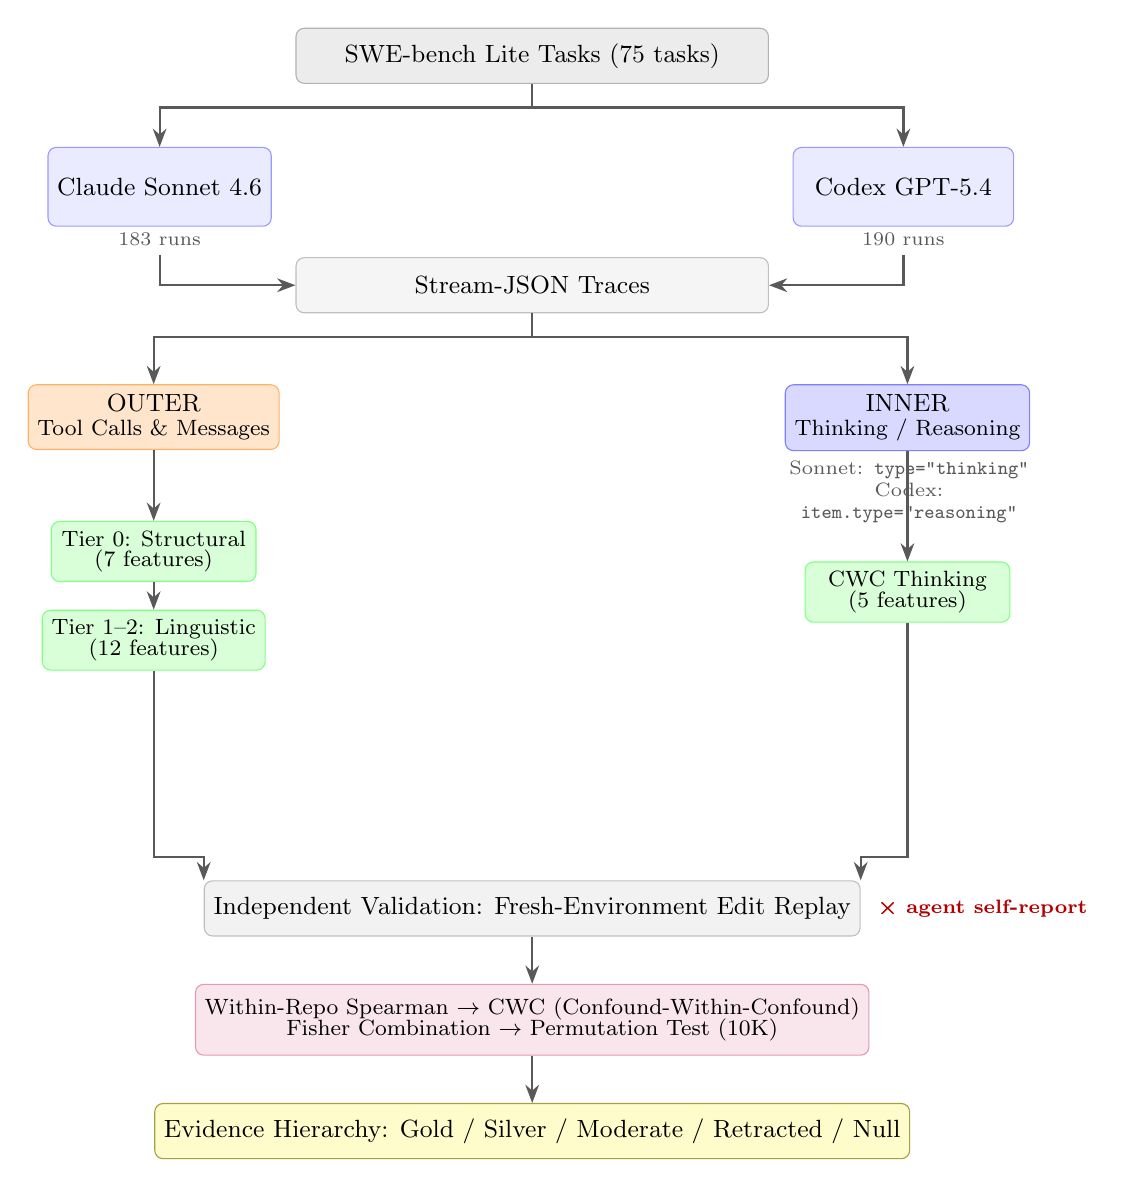
\begin{tikzpicture}[
    >=Stealth,
    node distance=0.6cm and 1.2cm,
    every node/.style={font=\small},
    box/.style={draw, rounded corners=3pt, minimum width=2.8cm, minimum height=0.7cm, align=center, font=\small},
    widebox/.style={draw, rounded corners=3pt, minimum width=6.0cm, minimum height=0.7cm, align=center, font=\small},
    taskbox/.style={box, fill=gray!15, draw=gray!60},
    agentbox/.style={box, fill=blue!8, draw=blue!40, minimum height=1.0cm},
    tracebox/.style={box, fill=gray!8, draw=gray!50},
    outerbox/.style={box, fill=orange!20, draw=orange!60},
    innerbox/.style={box, fill=blue!15, draw=blue!50},
    featbox/.style={box, fill=green!15, draw=green!50, font=\footnotesize},
    valbox/.style={widebox, fill=gray!10, draw=gray!50},
    statbox/.style={box, fill=purple!10, draw=purple!40, font=\footnotesize},
    evidbox/.style={widebox, fill=yellow!20, draw=yellow!60!black},
    annot/.style={font=\scriptsize, text=gray!70!black},
    arr/.style={->, thick, gray!70!black},
]

% ---- Task source ----
\node[taskbox, minimum width=6.0cm] (tasks) {SWE-bench Lite Tasks (75 tasks)};

% ---- Agent columns ----
\node[agentbox, below left=0.8cm and 0.3cm of tasks] (sonnet) {Claude Sonnet 4.6};
\node[annot, below=-0.05cm of sonnet] (sann) {183 runs};
\node[agentbox, below right=0.8cm and 0.3cm of tasks] (codex) {Codex GPT-5.4};
\node[annot, below=-0.05cm of codex] (cann) {190 runs};

\draw[arr] (tasks.south) -- ++(0,-0.3) -| (sonnet.north);
\draw[arr] (tasks.south) -- ++(0,-0.3) -| (codex.north);

% ---- Stream-JSON trace ----
\node[tracebox, minimum width=6.0cm, below=1.0cm of tasks, yshift=-1.2cm] (trace) {Stream-JSON Traces};
\draw[arr] (sann.south) |- (trace.west);
\draw[arr] (cann.south) |- (trace.east);

% ---- Outer / Inner split ----
\node[outerbox, below left=0.9cm and 0.2cm of trace, minimum width=2.6cm] (outer) {OUTER\\[-2pt]{\footnotesize Tool Calls \& Messages}};
\node[innerbox, below right=0.9cm and 0.2cm of trace, minimum width=2.6cm] (inner) {INNER\\[-2pt]{\footnotesize Thinking / Reasoning}};

\draw[arr] (trace.south) -- ++(0,-0.3) -| (outer.north);
\draw[arr] (trace.south) -- ++(0,-0.3) -| (inner.north);

% ---- Inner annotations ----
\node[annot, below=0.0cm of inner, text width=3.0cm, align=center] (innernote) {Sonnet: \texttt{type="thinking"}\\Codex: \texttt{item.type="reasoning"}};

% ---- Feature extraction boxes ----
\node[featbox, below=0.9cm of outer, minimum width=2.6cm] (tier0) {Tier 0: Structural\\[-2pt](7 features)};
\node[featbox, below=0.35cm of tier0, minimum width=2.6cm] (tier12) {Tier 1--2: Linguistic\\[-2pt](12 features)};
\node[featbox, below=1.4cm of inner, minimum width=2.6cm] (cwc) {CWC Thinking\\[-2pt](5 features)};

\draw[arr] (outer.south) -- (tier0.north);
\draw[arr] (tier0.south) -- (tier12.north);
\draw[arr] (inner.south) -- ++(0,-0.5) -- (cwc.north);

% ---- Independent Validation ----
\node[valbox, below=3.2cm of trace, yshift=-4.0cm] (val) {Independent Validation: Fresh-Environment Edit Replay};
\node[annot, right=0.1cm of val, text=red!70!black] (valx) {\bfseries\texttimes\ agent self-report};

% ---- Statistical pipeline ----
\node[statbox, below=0.6cm of val, minimum width=6.0cm, minimum height=0.9cm] (stats) {%
Within-Repo Spearman $\to$ CWC (Confound-Within-Confound)\\[-2pt]
Fisher Combination $\to$ Permutation Test (10K)};

\draw[arr] (tier12.south) |- ([yshift=0.3cm]val.north west) -- (val.north west);
\draw[arr] (cwc.south) |- ([yshift=0.3cm]val.north east) -- (val.north east);
\draw[arr] (val.south) -- (stats.north);

% ---- Evidence hierarchy ----
\node[evidbox, below=0.6cm of stats] (evid) {Evidence Hierarchy: Gold / Silver / Moderate / Retracted / Null};
\draw[arr] (stats.south) -- (evid.north);

\end{tikzpicture}
}
\caption{Behavioral exhaust mining pipeline. Two models (Sonnet 4.6, Codex GPT-5.4) solve SWE-bench tasks, producing stream-JSON traces containing both outer signals (tool calls, agent messages) and inner signals (thinking blocks). Sonnet produces extended thinking blocks (\texttt{type="thinking"}); Codex produces reasoning items (\texttt{item.type="reasoning"}). Both are labeled ``Inner'' in the diagram. Features are extracted at three tiers: structural (from tool-call sequences), linguistic (from reasoning text), and thinking-block features (from internal reasoning). Independent validation via fresh-environment edit replay provides ground truth labels; agent self-report is never used. Within-repo Spearman correlations are combined via Fisher's method (CWC---Confound-Within-Confound) and validated by permutation testing.}
\label{fig:architecture}
\end{figure*}

\subsection{Task Selection and Agent Configuration}

We selected 75 tasks from SWE-bench Lite \citep{jimenez2024swebench} spanning 9 Python repositories: django, sympy, pytest-dev, scikit-learn, pylint-dev, psf, sphinx-doc, pallets, and astropy.
Tasks were chosen to produce a blended pass rate near 50\%, providing balanced classes for correlation analysis.
Repository-level pass rates range from 0\% (scikit-learn, sphinx-doc, astropy) to 100\% (pallets), with the two largest repositories---sympy ($n = 87$ Sonnet runs, 41.4\% pass) and django ($n = 44$ Sonnet runs, 84.1\% pass)---providing the primary analytical strata.

Two models served as agents.
Claude Sonnet~4.6 was invoked via {\small\texttt{claude -p --model sonnet --output-format stream-json --verbose}}, producing 183 validated runs across all 75 tasks.
Codex GPT-5.4 was invoked via \texttt{codex exec}, producing 190 validated runs across 70 of the 75 tasks (five tasks were Sonnet-only due to infrastructure constraints).
Both agents received the bug description and were instructed to fix it and run tests.
No intervention, gating, or prompt augmentation was applied.
Each run had a 30-minute wall-clock timeout.

Full stream-json traces were captured and stored in SQLite (WAL mode).
Each trace record contains every tool call (tool name, parameters, result, \texttt{is\_error} flag), reasoning text preceding each tool call (when present), and sequence numbers.
Sonnet runs produced approximately 3,600 state-modifying tool calls total, of which 28\% had per-call reasoning annotations.
Codex runs had 60.1\% per-call reasoning coverage.

\subsection{Independent Validation}

Agent self-report was not used for outcome labeling.
We discovered that using the agent's own test output as ground truth inflated three features to statistical significance that disappeared under independent validation.
The agent has incentive structure (implicit in its training) to report success; its self-assessment cannot be treated as ground truth.

Independent validation proceeds as follows: (1)~copy the original repository to a fresh temporary directory; (2)~extract all Write and Edit operations from the raw stream-json trace; (3)~apply these edits to the fresh copy in sequence order; (4)~create a Python~3.10 virtual environment with SWE-bench-pinned dependencies; (5)~run the specific \texttt{FAIL\_TO\_PASS} tests from the SWE-bench dataset; (6)~label the run as pass or fail based on the test exit code.

Of the 395 total runs attempted, 373 received validation labels.
Of these, 28 runs (26 Codex, 2 Sonnet) had infrastructure failures that prevented definitive pass/fail determination; these are included in the validated count but excluded from all correlation analyses, leaving 345 runs with definitive outcomes (181 Sonnet, 164 Codex) as the analysis dataset.

\subsection{Behavioral Feature Extraction}

We extract 24 primary features organized into three tiers plus a set of thinking-block features, and 3 supplementary features tested during null-result analysis (27 total; all features are defined in Appendix~\ref{app:features}).
Here we describe the three tiers and the aggregation method.

\textbf{Tier~0---Structural features} are computed from the tool-call sequence alone, with no text analysis.
These include error-streak length, early error rate, the normalized position of the first code edit, file count, edit churn, test invocation count, and total call count (used as a control variable).

\textbf{Tier~1---Linguistic features} are computed from per-call reasoning text using the \citet{hyland2005metadiscourse} hedging lexicon and related marker sets.
Features in this tier measure hedge-word density, mean reasoning length per call, backtrack marker density, verification phrase density, and planning phrase density.

\textbf{Tier~2---Domain-specific features} are computed from per-call reasoning text using marker sets developed for this study.
These capture metacognitive self-correction, tentative language, insight phrases, contrastive markers (``however,'' ``but,'' ``instead''), self-directive language (``let me,'' ``I should''), and backtick identifier density.
One cross-tier feature, reasoning-to-action alignment (\rtalign{} in tables), measures whether the reasoning text preceding an edit names the file about to be edited.

\textbf{CWC thinking features} are extracted from internal reasoning blocks (see Section~\ref{sec:thinking}) rather than from per-call reasoning annotations.
These measure diagnostic precision (code-specific reference density), reasoning clarity (diagnostic precision minus confusion score), function reference density, compatibility/environment sentence fraction, and strategy pivot density.

The 24 primary features and the feature extraction pipeline serve as infrastructure for this study.
The pipeline computes features from existing trace data with zero API overhead; all features use per-call mean aggregation to control for the task-length confound (see below).

\textbf{Aggregation method.}
All linguistic and domain-specific features use mean aggregation: per-call values are computed as per-token densities, then averaged across calls within a run.
We do not use sum aggregation.
This choice controls for the task-length confound: failing runs produce 35\% more state-modifying tool calls than passing runs (mean 22.6 vs.\ 16.7).
Any feature aggregated by summation would be mechanically correlated with failure through call count alone.
The task-length confound suppressed the metacognitive signal in raw sum correlations ($\rho$ rose from $+0.308$ to $+0.494$ after switching to mean aggregation with partial correlation controlling for \feat{n\_calls}).

\subsection{Thinking Block Extraction}
\label{sec:thinking}

Both models produce internal reasoning content that is hidden from the user but present in the stream-json trace.
Sonnet~4.6 produces extended thinking blocks (content blocks with \texttt{type\allowbreak{}="thinking"}, text in the \texttt{"thinking"} key).
Codex GPT-5.4 produces reasoning items (items with \texttt{item.type\allowbreak{}="reasoning"}, text in the \texttt{"text"} key).
Both models have 100\% thinking-block coverage: every validated run contains internal reasoning content.
Sonnet produced approximately 2.1 million characters of internal reasoning across 183 runs (mean ${\sim}$11,700 chars/run, median 2,758 chars/run, right-skewed).
Codex produced approximately 1.1 million characters across 190 runs (mean 5,754 chars/run, median 5,548 chars/run, more uniform distribution).

\textbf{Parser bug discovery and correction.}
The original trace collector read \texttt{block.get("text")} for all content blocks, including Sonnet thinking blocks.
Because Sonnet stores internal reasoning in the \texttt{"thinking"} key rather than \texttt{"text"}, this returned empty strings for all thinking blocks.
The original 23-feature analysis (Tiers~0--2) therefore operated entirely on agent messages, not internal thinking.
After fixing the parser, thinking block content was recovered for all 183 Sonnet runs, and the five CWC thinking features were computed from this recovered content.
This bug had the incidental benefit of keeping the Tier~0--2 analysis cleanly separated from thinking block content; the original results remain valid.

\subsection{Statistical Methods}
\label{sec:stats}

The primary analytical challenge is repository-level heterogeneity: django passes at 84\% while sympy passes at 41\%.
Pooling across repositories produces spurious correlations whenever a feature's distribution varies by repository.
We address this through a multi-layer framework.

\textbf{Within-repo Spearman correlations.}
We compute Spearman rank correlations between each feature and binary success (0/1) separately within django and sympy, the two repositories with sufficient sample size (Sonnet: django $n = 44$, sympy $n = 87$; Codex: django $n = 59$, sympy $n = 78$).
All correlations use a custom implementation with correct tie handling and exact $p$-values from the regularized incomplete beta function.

\textbf{Fisher's combined $p$-value (CWC decomposition).}
The exact algorithm is: (1)~compute within-repo Spearman $\rho$ and two-tailed $p$-value for each major repository (sympy, django), (2)~verify direction consistency across repos, (3)~combine $p$-values via Fisher's method ($\chi^2 = -2 \sum \log(p_i)$, $df = 2k$) only for features with consistent direction, (4)~compute sample-size-weighted average $\rho$.
A feature must show a consistent direction across repos to survive.

\textbf{Within-repo permutation test.}
For each of 10,000 permutations, success labels are shuffled independently within each repository, preserving repo-level pass rates.
The test statistic is the weighted average mean difference (pass minus fail) across repos.
This test controls for between-repo confounds but does not control for within-repo task difficulty variation.
At the tails, permutation $p$-values have limited precision; the smallest achievable value with 10,000 permutations is 0.0001.
We interpret these values as evidence of crossing the $\alpha = 0.05$ threshold rather than as precise tail probabilities.

\textbf{Cross-model comparison.}
For each feature, we compare the direction and significance of within-repo Spearman correlations between Sonnet and Codex on the 70 shared tasks.
Features are classified as cross-model (same significant direction in both), model-specific (significant in one only), or polarity-flipped (significant in both with opposite signs).

\textbf{Multiple comparison correction.}
Bonferroni correction at $\alpha/23 = 0.0022$ is applied to the pooled analysis (23 features excluding \feat{n\_calls}, which serves as a control).
The CWC decomposition and permutation tests provide independent multiple-comparison safeguards: the CWC approach reduces the effective number of comparisons by requiring within-repo consistency, and the permutation test provides a non-parametric $p$-value that accounts for the full feature-selection procedure within each permutation.
We report results under both Bonferroni and Benjamini--Hochberg FDR ($q = 0.05$) corrections.
For the CWC Fisher-combined $p$-values, all five surviving features (\feat{first\_edit\_position}, \feat{deliberation\_length}, \feat{backtrack\_count}, \feat{early\_error\_rate}, \feat{fail\_streak\_max}) survive under both Bonferroni and BH-FDR.
For within-repo Spearman in sympy alone (23 features), only \feat{backtrack\_count} ($p = 0.0006$) survives either correction; the remaining features survive only through the CWC combination, which aggregates evidence across repositories.
The convergence of Bonferroni and BH-FDR for the CWC results indicates that the multiple-comparison correction choice does not affect the paper's conclusions.

\textbf{What the permutation test controls and does not control.}
The within-repo permutation test eliminates between-repo confounds by construction: because labels are shuffled within each repo independently, any feature whose apparent association with success is driven by repo-level pass rate differences will not survive.
This is precisely the confound that inflated \rtalign{} to apparent significance in the pooled analysis (Section~\ref{sec:retraction}).
However, the test does not control for within-repo task difficulty variation.
If a feature correlates with task difficulty within a repository (e.g., harder tasks produce longer error streaks and also fail more often), the permutation test will still find it significant.
A within-task permutation on mixed-outcome tasks partially addresses this but is limited by the small number of such tasks (7 for Sonnet, 5 for Codex).
Given the small sample (7 tasks, 35 runs for Sonnet; 5 tasks, 18 runs for Codex), the within-task result should be treated as suggestive rather than confirmatory.


% ============================================================
\section{Results}
\label{sec:results}

\subsection{Aggregate Performance}

Table~\ref{tab:aggregate} summarizes the validated dataset across both models.

\begin{table}[t]
\centering
\caption{Aggregate performance by model.}
\label{tab:aggregate}
\begin{tabular}{lccc}
\toprule
\textbf{Model} & \textbf{Validated Runs} & \textbf{Pass Rate} & \textbf{Unique Tasks} \\
\midrule
Sonnet 4.6     & 183 & 49.2\% (90/183) & 75 \\
Codex GPT-5.4  & 190 & 41.1\% (78/190) & 70 \\
\midrule
\textbf{Combined} & \textbf{373} & \textbf{45.0\%} & \textbf{75} \\
\bottomrule
\end{tabular}
\end{table}

Of the 190 validated Codex runs, 26 had infrastructure failures during validation (environment setup crashes unrelated to the agent's code changes) and received no definitive pass/fail outcome.
These runs are included in the validated count but excluded from all feature correlation analyses.
Pass rates reported in Table~\ref{tab:aggregate} use the full validated denominator (Sonnet: 90/183 = 49.2\%; Codex: 78/190 = 41.1\%); on runs with definitive outcomes, the rates are 90/181 = 49.7\% and 78/164 = 47.6\% respectively.
Two Sonnet runs were similarly unrecoverable.
All Spearman correlations, CWC analyses, and permutation tests use only runs with definitive outcomes ($n = 181$ Sonnet, $n = 164$ Codex, total $n = 345$).

(Note: Three pass rates are reported for Sonnet because they use different denominators: 90/183 = 49.2\% includes all validated runs; 90/181 = 49.7\% excludes 2 unrecoverable infrastructure failures; 88/178 = 49.4\% uses only the 70-task matched subset.
All correlation analyses use the $n = 181$ definitive-outcome set.)

The exclusion of 28 infrastructure-failure runs reduces Codex power by 14\% (190 to 164 runs, sympy 84 to 78).
Codex features that were marginal at the larger sample size should be interpreted with this power reduction in mind.

All cross-model comparisons use the matched set of 70 shared tasks.
On this set, Sonnet passes 49.4\% of runs (88/178) and Codex passes 41.1\% (78/190), an 8.3 percentage-point gap present in both major repositories.

\begin{table}[t]
\centering
\caption{Task-level agreement matrix (70 shared tasks, majority vote).}
\label{tab:agreement}
\begin{tabular}{lcc}
\toprule
 & \textbf{Codex Pass} & \textbf{Codex Fail} \\
\midrule
\textbf{Sonnet Pass} & 27 & 7 \\
\textbf{Sonnet Fail} & 2 & 34 \\
\bottomrule
\end{tabular}
\end{table}

Agreement: 87.1\% (61/70; ties broken toward pass), Cohen's $\kappa = 0.742$ (substantial).
Django shows perfect agreement (23/23 tasks).
Sympy shows the most disagreement (25/30, 83\%), consistent with its balanced difficulty providing the most room for model-specific differences.
Despite this high agreement on \emph{which} tasks they solve, the models' behavioral signatures diverge sharply, as the following sections demonstrate.


\subsection{Features Surviving CWC and Permutation}
\label{sec:features}

We applied a three-stage filter: (1)~within-repo Spearman correlation at $p < 0.05$ in at least one major repository, (2)~Fisher-combined within-repo $p$-value (CWC) at $p < 0.05$, and (3)~within-repo permutation test (10,000 permutations) at $p < 0.05$.
Table~\ref{tab:hierarchy} presents the evidence hierarchy.

We define three tiers based on statistical survival criteria: \textbf{Gold} requires significant same-direction association in both models within the same repository.
\textbf{Silver} requires CWC survival ($p < 0.05$) and permutation survival ($p < 0.05$) within one model.
\textbf{Moderate} requires CWC and permutation survival with a noted caveat (failed cross-wave replication or single-model significance).

\begin{table}[t]
\centering
\caption{Evidence hierarchy for behavioral features.}
\label{tab:hierarchy}
\small
\begin{adjustbox}{max width=\textwidth}
\begin{tabular}{p{2.2cm}p{4.2cm}p{7.5cm}}
\toprule
\textbf{Level} & \textbf{Features} & \textbf{Key Evidence} \\
\midrule
\textbf{Gold} (both models, structural)
  & \feat{fail\_streak\_max}, \feat{early\_error\_rate}
  & Sonnet/sympy: $\rho = {-}0.294$ ($p = 0.006$), ${-}0.273$ ($p = 0.011$). Codex/sympy: $\rho = {-}0.296$ ($p = 0.009$), ${-}0.282$ ($p = 0.012$). Same direction, both significant. \\
\midrule
\textbf{Silver} (model-specific, all tests)
  & \feat{deliberation\_length} (Sonnet), \feat{think\_t\_compat\_fraction} (Codex)
  & Sonnet: CWC $p = 0.003$, perm $p = 0.0004$. Codex: CWC $p = 0.010$, perm $p = 0.006$. \\
\midrule
\textbf{Moderate} (CWC + perm, weaker)
  & \feat{first\_edit\_position} (Sonnet), \feat{instead\_contrast\_density} (Codex)
  & Sonnet: CWC $p = 0.001$, perm $p = 0.001$, but no wave-2 replication. Codex: CWC $p = 0.013$, perm $p = 0.007$. \\
\midrule
\textbf{Retracted}
  & \rtalign{}
  & Perm $p = 0.35$; between-repo confound. See Section~\ref{sec:retraction}. \\
\midrule
\textbf{Null}
  & \feat{hedging\_score}, \feat{verification\_score}, \feat{planning\_score}, \feat{precision\_naming\_score}
  & No signal in any analysis (see Section~\ref{sec:null}). \\
\bottomrule
\end{tabular}
\end{adjustbox}
\end{table}

The Gold-tier features are both Tier~0 structural measures---they require no text analysis, only the sequence of tool-call error flags.
No linguistic feature is significantly associated with success in the same direction for both models.

Two caveats apply to the evidence hierarchy.
First, the two Gold-tier features are correlated ($r = 0.64$), suggesting they may measure a single underlying construct---the agent's early encounter with environmental obstacles---rather than two independent signals.
Second, among Sonnet-specific features, \feat{backtrack\_count} and \feat{metacognitive\_density} correlate at $r = 0.90$, meaning they are effectively interchangeable; we retain both in the feature table but treat them as a single signal in interpretation.

\begin{table}[t]
\centering
\caption{Within-repo Spearman correlations for surviving features, cross-model comparison. Only features significant ($p < 0.05$) in at least one cell are shown. Cells marked ``--'' indicate non-significant results ($p > 0.05$).}
\label{tab:spearman}
\small
\begin{adjustbox}{max width=\textwidth}
\setlength{\tabcolsep}{3pt}
\begin{tabular}{lcccccccc}
\toprule
 & \multicolumn{2}{c}{\textbf{Sonnet/sympy}} & \multicolumn{2}{c}{\textbf{Sonnet/django}} & \multicolumn{2}{c}{\textbf{Codex/sympy}} & \multicolumn{2}{c}{\textbf{Codex/django}} \\
\cmidrule(lr){2-3}\cmidrule(lr){4-5}\cmidrule(lr){6-7}\cmidrule(lr){8-9}
\textbf{Feature} & $\rho$ & $p$ & $\rho$ & $p$ & $\rho$ & $p$ & $\rho$ & $p$ \\
 & \multicolumn{2}{c}{($n{=}87$)} & \multicolumn{2}{c}{($n{=}44$)} & \multicolumn{2}{c}{($n{=}78$)} & \multicolumn{2}{c}{($n{=}59$)} \\
\midrule
\feat{fail\_streak\_max}           & $-$0.294 & 0.006 & -- & n.s. & $-$0.296 & 0.009 & -- & n.s. \\
\feat{early\_error\_rate}          & $-$0.273 & 0.011 & -- & n.s. & $-$0.282 & 0.012 & $-$0.322 & 0.013 \\
\feat{deliberation\_length}        & $+$0.214 & 0.046 & $+$0.396 & 0.008 & -- & n.s. & -- & n.s. \\
\feat{instead\_contrast\_density}  & $+$0.282 & 0.008 & -- & n.s. & $-$0.264 & 0.020 & -- & n.s. \\
\feat{think\_t\_compat\_fraction}  & -- & n.s. & -- & n.s. & $-$0.323 & 0.004 & -- & n.s. \\
\feat{backtrack\_count}            & $+$0.359 & 0.0006 & -- & n.s. & $-$0.108 & ${>}0.05$ & -- & n.s. \\
\feat{first\_edit\_position}       & -- & n.s. & $+$0.493 & 0.0007 & -- & n.s. & -- & n.s. \\
\bottomrule
\end{tabular}
\end{adjustbox}
\end{table}

Sonnet's django results for \feat{early\_error\_rate} are individually non-significant, likely a ceiling effect from the 84\% pass rate compressing the failure distribution.
Codex/django (73.2\% pass rate, $n = 59$) retains enough failures for the structural feature to reach significance.

\textbf{Partial correlation sensitivity check.}
Within Sonnet/sympy, we computed Spearman partial correlations controlling for \feat{n\_calls} (total tool calls) to assess whether the task-length confound is fully controlled by mean aggregation.
Results are mixed: \feat{early\_error\_rate} retains significance ($\rho_{\text{partial}} = -0.232$, $p = 0.031$), but \feat{deliberation\_length} drops to non-significance ($\rho_{\text{partial}} = 0.144$, $p = 0.183$), and \feat{fail\_streak\_max} becomes marginal ($\rho_{\text{partial}} = -0.186$, $p = 0.086$).
This suggests that within sympy, the \feat{deliberation\_length} association may be partly mediated by task length---runs with more calls (which tend to fail) may have mechanically lower per-call deliberation.
However, \feat{deliberation\_length} survives the CWC pipeline (which combines evidence across repos) and the within-repo permutation test ($p = 0.0004$), which are more robust tests than within-sympy partial correlation alone.
We interpret the partial correlation as a caveat on the feature's within-repo robustness, not a retraction.


\subsubsection{Retraction: Reasoning-to-Action Alignment}
\label{sec:retraction}

The original analysis reported \rtalign{} as the strongest Bonferroni survivor (coefficient $= +1.133$, raw $p = 0.00018$, Bonferroni-adjusted $p = 0.004$).
This feature measures whether the agent's reasoning text mentions the file it is about to edit.

The finding does not survive the within-repo permutation test ($p = 0.35$).
The pooled effect was inflated by between-repo confounding: repositories where the agent tends to name files (e.g., django, with its explicit file structure) also happen to have high pass rates.
Once labels are shuffled within each repo, the association disappears.

We report this retraction prominently because it illustrates why the CWC methodology matters.
A feature that appears highly significant in a pooled analysis ($p = 0.00018$) can be entirely driven by confound structure.
The permutation test, by preserving repo-level pass rates, exposes the confound.
This is a methodological success, not a failure: the pipeline's self-correction mechanism works as intended.


\subsection{The Polarity Flip}
\label{sec:polarity}

One feature shows a confirmed polarity flip---significant in both models within the same repository, with opposite signs.

\begin{table}[t]
\centering
\caption{Polarity flips in sympy.}
\label{tab:polarity}
\small
\begin{tabular}{lccccc}
\toprule
\textbf{Feature} & \textbf{Sonnet $\rho$} & \textbf{Sonnet $p$} & \textbf{Codex $\rho$} & \textbf{Codex $p$} & \textbf{Status} \\
 & ($n{=}87$) & & ($n{=}78$) & & \\
\midrule
\feat{instead\_contrast\_density} & $+$0.282 & 0.008 & $-$0.264 & 0.020 & \textbf{Confirmed flip} \\
\feat{backtrack\_count}           & $+$0.359 & 0.0006 & $-$0.108 & ${>}0.05$ & Suggestive (Codex n.s.) \\
\feat{metacognitive\_density}     & $+$0.138 & ${>}0.05$ & $-$0.261 & 0.021 & Suggestive (Sonnet n.s.) \\
\bottomrule
\end{tabular}
\end{table}

Note: \feat{think\_t\_compat\_fraction} (environment compatibility language in thinking blocks) is exclusively a Codex feature ($\rho = -0.323$, $p = 0.004$ in Codex/sympy) with no significant association in Sonnet. It does not appear in the polarity-flip table because it is model-specific, not opposite-direction.

The confirmed flip on \feat{instead\_contrast\_density} means that words like ``however,'' ``but,'' and ``instead'' are associated with success in Sonnet but failure in Codex, within the same task repository.
Qualitative inspection suggests the mechanism differs: in Sonnet, contrastive markers appear within diagnostic reasoning (``The function returns X, but the expected behavior is Y''), narrowing the gap between observed and expected behavior.
In Codex, the same markers appear within strategic pivots (``However, let me try a different approach instead''), signaling abandonment of one approach for another.
This interpretation is post-hoc and based on qualitative inspection of a small number of examples; it should be treated as a hypothesis for future systematic coding analysis, not as an established finding.


\subsection{Thinking/Message Crossover}
\label{sec:crossover}

Correcting the parser bug described in Section~\ref{sec:thinking} revealed that the same lexical feature carries opposite signal depending on which layer it is extracted from.

\begin{table}[t]
\centering
\caption{The ``actually'' layer-dependent polarity reversal in Sonnet.}
\label{tab:actually}
\small
\begin{tabular}{@{}llrrrl@{}}
\toprule
\textbf{Layer} & \textbf{Feature} & \textbf{$\rho$} & \textbf{95\% CI} & \textbf{Perm.\ $p$} & \textbf{Interpretation} \\
\midrule
Thinking & ``actually'' & $-0.253$ & $[-0.384, -0.112]$ & 0.436 & Genuine confusion \\
Messages & ``actually'' & $+0.494$ & $[+0.376, +0.596]$ & --- & Performative correction \\
\bottomrule
\end{tabular}
\end{table}

Internal reasoning is present in every run (183/183 Sonnet runs, approximately 2.1M total characters, mean ${\sim}$11,700 chars/run) and is roughly 10$\times$ longer than the polished agent messages (approximately 1,200 chars/run).
Two additional features show a similar layer-dependent polarity pattern:

\begin{table}[t]
\centering
\caption{Layer-specific feature associations (Sonnet, $n = 183$).}
\label{tab:layer}
\small
\begin{tabular}{lccccc}
\toprule
\textbf{Feature} & \textbf{Think.\ $\rho$} & \textbf{Think.\ $p$} & \textbf{Think.\ perm $p$} & \textbf{Msg.\ $\rho$} & \textbf{Msg.\ $p$} \\
\midrule
\feat{tentative\_density} & $-$0.346 & 0.003 & \textbf{0.0012} & $-$0.204 & 0.083 \\
\feat{insight\_density}   & $\approx 0$ & n.s. & -- & $+$0.248 & 0.034 \\
\bottomrule
\end{tabular}
\end{table}

Internal doubt (\feat{tentative\_density} in thinking: $\rho = -0.346$, $p = 0.003$) is diagnostic; the same feature in messages does not survive ($p = 0.083$).
Expressed correction (\feat{insight\_density} in messages: $\rho = +0.248$, $p = 0.034$) is diagnostic; the thinking-layer version is near zero.
The two layers carry structurally different information: \textbf{internal doubt lives in thinking; expressed correction lives in messages}.
Any feature pipeline that conflates the layers will cancel real signals.

We subjected the thinking-block features to the same within-repo permutation test applied to all other features (10,000 permutations, labels shuffled within repo).
\feat{tentative\_density} in thinking blocks survives (permutation $p = 0.0012$): internal tentative language (``let me try,'' ``maybe,'' ``not sure'') is significantly more dense in failing runs' thinking blocks, confirming that internal doubt is a genuine behavioral signal.
However, \feat{actually\_density} in thinking blocks does not survive permutation ($p = 0.436$).
The ``actually'' reversal reported in Table~\ref{tab:actually}---the most vivid example of the crossover---is a within-sample observation that does not generalize under confound control.
We retain it in Table~\ref{tab:actually} as an illustrative example but note that it should be treated as a hypothesis rather than a confirmed finding.


\subsection{Trajectory Degradation}
\label{sec:degradation}

Signal quality degrades over the trajectory.
We split each run into thirds by normalized call position and computed feature-outcome associations within each segment.

\begin{table}[t]
\centering
\caption{Feature-outcome association by trajectory position (Sonnet, $n = 183$). $\dagger$RETRACTED: \rtalign{} was retracted after within-repo permutation testing revealed between-repository confounding (Section~\ref{sec:retraction}). It is included here for comparison only.}
\label{tab:degradation}
\small
\begin{tabular}{lcccc}
\toprule
\textbf{Trajectory position} & \textbf{delib.\ $\rho$} & \textbf{delib.\ $p$} & \textbf{align.$\dagger$\ $\rho$} & \textbf{align.$\dagger$\ $p$} \\
\midrule
Early (0--33\%)  & $+$0.180 & 0.016 & $+$0.242 & 0.001 \\
Mid (33--67\%)   & $+$0.166 & 0.028 & $+$0.165 & 0.029 \\
Late (67--100\%) & $+$0.038 & 0.615 & $+$0.026 & 0.735 \\
\bottomrule
\end{tabular}
\end{table}

Both features are associated with success in the early and middle trajectory segments and are completely non-associated in the late segment.
By the final third, the agent has either found the fix or committed to a wrong approach; reasoning quality no longer discriminates.
The implication for gating is that a behavioral gate should focus on early and mid-trajectory decisions.
Late-trajectory gating based on reasoning features is uninformative.
Trajectory degradation analysis for structural features (\feat{fail\_streak\_max}, \feat{early\_error\_rate}) is consistent in direction but not tabulated here; see supplementary materials.

\citet{shojaee2025illusion} observe accuracy collapse in reasoning models beyond certain complexity thresholds, consistent with this trajectory degradation pattern: as the agent's context fills with accumulated decisions and outputs, the behavioral signal-to-noise ratio declines.

\begin{figure}[t]
\centering
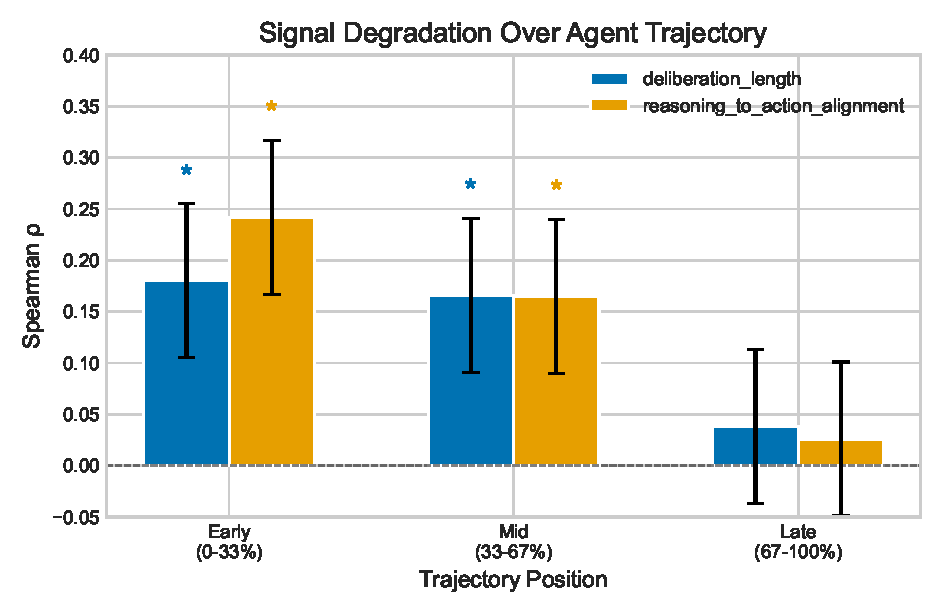
\includegraphics[width=0.85\textwidth]{figures/fig1_trajectory_degradation.pdf}
\caption{Trajectory degradation of behavioral signal quality. Feature-outcome associations (Spearman $\rho$) are computed within early (0--33\%), mid (33--67\%), and late (67--100\%) segments of the agent's trajectory. Both deliberation length and alignment show significant associations in early and mid segments but collapse to near-zero in the late segment, indicating that behavioral monitoring should focus on early-trajectory decisions.}
\label{fig:trajectory}
\end{figure}


\subsection{The Interaction Effect}
\label{sec:interaction}

In Sonnet/sympy ($n = 87$), \feat{deliberation\_length} and \feat{think\_diagnostic\_precision} interact to produce a nonlinear association with success.
We split both features at their per-repo medians to form four quadrants.

A methodological note: \feat{deliberation\_length} is computed from per-call reasoning text (present in 28\% of Sonnet calls), while \feat{think\_diagnostic\_precision} is computed from thinking blocks (present in 100\% of runs).
The interaction therefore combines features with different measurement granularity.

\begin{table}[t]
\centering
\caption{Quadrant analysis: deliberation $\times$ diagnostic precision (Sonnet/sympy).}
\label{tab:interaction}
\begin{tabular}{llcc}
\toprule
\textbf{Deliberation} & \textbf{Diagnostic Precision} & \textbf{Pass Rate} & $n$ \\
\midrule
High & High & 73\% & 22 \\
High & Low  & 23\% & 22 \\
Low  & High & 32\% & 22 \\
Low  & Low  & 38\% & 21 \\
\bottomrule
\end{tabular}
\end{table}

The interaction bonus is $+0.56$, computed as the excess of the high-high cell over the additive expectation from main effects ($0.73 - (0.23 + 0.32 - 0.38) = 0.56$).
Neither feature alone is sufficient: an agent that deliberates extensively without diagnostic precision (23\%) performs worse than one that barely deliberates at all (38\%).
But an agent that reasons deeply \emph{and} precisely about code artifacts succeeds 73\% of the time.
In Codex/sympy, the same interaction is much weaker ($+0.13$), consistent with Codex's reasoning blocks being more strategic than diagnostic.

\textbf{Caveat.}
This analysis is exploratory.
Each quadrant contains approximately 22 runs.
The interaction has not been tested with a formal interaction model.
Median-split analyses are known to inflate apparent interaction effects \citep{maccallum2002practice}.
The $+0.56$ interaction bonus should be interpreted with this caveat; a formal logistic regression with continuous interaction terms is needed to confirm the effect size.
These results motivate a formal interaction model in future work but should not be treated as confirmed.

\begin{figure}[t]
\centering
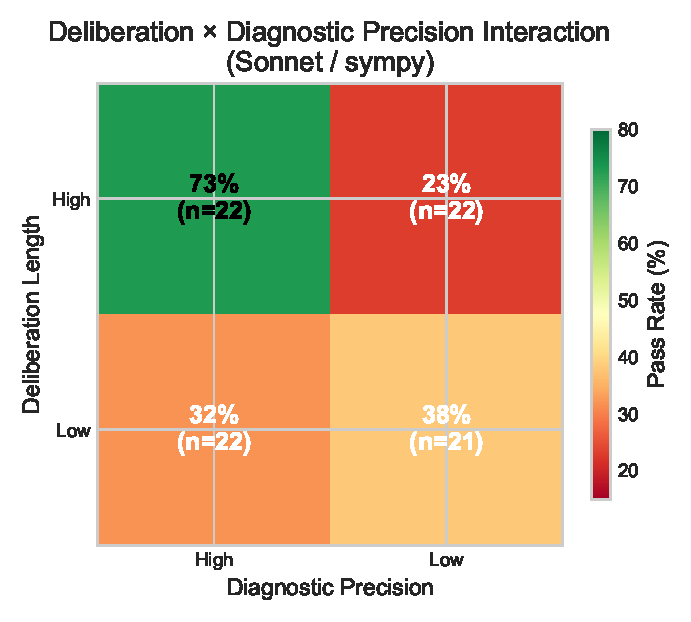
\includegraphics[width=0.85\textwidth]{figures/fig2_interaction_heatmap.pdf}
\caption{Interaction between deliberation length and diagnostic precision (Sonnet/sympy, $n = 87$). The high-deliberation, high-precision quadrant yields a 73\% pass rate---far exceeding either feature alone (23--32\%). The interaction bonus of $+0.56$ suggests that length without precision may indicate unproductive rumination rather than careful analysis, though the small cell sizes ($n \approx 22$) warrant caution.}
\label{fig:interaction}
\end{figure}


\subsection{Null Results}
\label{sec:null}

Seven features showed no meaningful association with success in any analysis.
We report these because understanding what does not work is as informative as understanding what does.
Three supplementary features (\feat{recovery\_rate}, \feat{fail\_then\_switch\_rate}, \feat{causal\_density}) were tested during this analysis but are not part of the 24 primary features; they are defined in Appendix~\ref{app:features}.

\begin{table}[t]
\centering
\caption{Features with null results. Supplementary features marked with *.}
\label{tab:null}
\small
\begin{tabular}{lcccp{4.5cm}}
\toprule
\textbf{Feature} & \textbf{Expected} & \textbf{Obs.\ $\rho$} & $p$ & \textbf{Reason for Failure} \\
\midrule
\feat{hedging\_score} (Hyland, 209 terms) & Negative & $\approx 0$ & 0.60 & Sonnet does not use academic hedge words when coding. \\
\feat{verification\_score}   & Negative & $+$0.02 & n.s. & Verification language is ubiquitous regardless of outcome. \\
\feat{planning\_score}       & Negative & $+$0.09 & n.s. & Sequential discourse markers are default style in both pass and fail. \\
\feat{precision\_naming\_score} & Positive & $+$0.04 & n.s. & Backtick identifiers are universal in code reasoning. No variance to exploit. \\
\feat{recovery\_rate}*       & Positive & $-$0.15 & n.s. & Dominated by infrastructure noise, not diagnostic quality. \\
\feat{fail\_then\_switch\_rate}* & Positive & $-$0.37 & -- & Tool-switching after errors is associated with flailing, not principled diagnosis. \\
\feat{causal\_density}*      & Positive & $-$0.03 & n.s. & General discourse markers with no task-success signal. \\
\bottomrule
\end{tabular}
\end{table}

The random noise control column returned $p = 0.52$, confirming that the pipeline does not produce spurious significant results.

The Hyland hedging null is the most theoretically consequential.
Academic hedging vocabulary---the foundation of most linguistic uncertainty research---carries zero signal in agent reasoning traces.
Agent uncertainty, to the extent it is linguistically expressed, appears through domain-specific structural markers, not through the modal expressions that characterize academic prose.

The failure of Hyland hedging in coding traces likely reflects a register difference: coding agents operate in a technical register where uncertainty is expressed through structural behaviors (re-reading code, running tests, exploring alternative approaches) rather than through the modal expressions (``might,'' ``could,'' ``arguably'') that characterize academic prose.
Multi-turn agentic interaction may also suppress hedging: unlike single-pass QA, the agent can resolve uncertainty by taking an action (running a test) rather than expressing it verbally.


\subsection{Cross-Wave Stability}

Features were tested for replication across two independently collected waves: the pilot wave ($n = 103$ Sonnet runs) and the protocol wave ($n = 77$ Sonnet runs, collected under a locked protocol with pre-registered task set).

\begin{table}[t]
\centering
\caption{Cross-wave replication (Sonnet). $\dagger$RETRACTED (permutation $p = 0.35$; Section~\ref{sec:retraction}).}
\label{tab:crosswave}
\small
\begin{tabular}{lccccl}
\toprule
\textbf{Feature} & \textbf{Pilot $\rho$} & \textbf{Pilot $p$} & \textbf{Protocol $\rho$} & \textbf{Protocol $p$} & \textbf{Replicates?} \\
 & ($n{=}103$) & & ($n{=}77$) & & \\
\midrule
\feat{deliberation\_length} & $+$0.320 & 0.001 & $+$0.273 & 0.016 & \textbf{Yes} \\
\rtalign{}$\dagger$ & $+$0.300 & 0.002 & $+$0.285 & 0.012 & $\dagger$RETRACTED \\
\feat{first\_edit\_position} & $+$0.241 & 0.014 & $+$0.039 & 0.736 & \textbf{No} \\
\bottomrule
\end{tabular}
\end{table}

\feat{deliberation\_length} replicates across both waves, making it the most robust Sonnet-specific finding.
\feat{first\_edit\_position} does not replicate in wave~2 ($\rho = +0.039$, $p = 0.736$), which is why it is classified as Moderate in Table~\ref{tab:hierarchy} despite surviving CWC and permutation.
\rtalign{} shows apparent cross-wave replication but is retracted on permutation grounds (Section~\ref{sec:retraction})---cross-wave consistency does not protect against a confound present in both waves.


\subsection{Held-Out Predictive Evaluation}

To bridge the gap between observed associations and predictive utility, we evaluate a leave-one-task-out cross-validation with nested feature selection.
For each held-out task, features are selected from the training set only (within-repo Spearman $|\rho| > 0.15$ and $p < 0.10$ in at least one major repository), avoiding the post-selection optimism that would arise from selecting features on the full dataset.
A logistic regression is trained on the selected features and evaluated on the held-out task's runs.

For Sonnet ($n = 181$ independently validated runs across 73 tasks), nested LOO-CV yields AUC = 0.569 (accuracy 56.9\%, base rate 49.7\%, 95\% bootstrap CI [0.489, 0.656], permutation $p = 0.064$).
For Codex ($n = 164$ runs across 65 tasks), AUC = 0.634 (accuracy 64.0\%, base rate 47.6\%, 95\% bootstrap CI [0.547, 0.720], permutation $p < 0.001$).

The divergence between models is interpretable.
Codex's primary features---the two Gold-tier structural measures (\feat{fail\_streak\_max}, \feat{early\_error\_rate})---are selected in 100\% of folds and carry robust out-of-sample signal.
Sonnet's linguistic features (\feat{deliberation\_length}, \feat{back\-track\_count}) are also stably selected (100\% of folds) but add less predictive power beyond the structural features.
The Sonnet result is marginal ($p = 0.064$), confirming that post-selection optimism inflated our earlier non-nested estimate (AUC = 0.624).
The Codex result is highly significant ($p < 0.001$), demonstrating that structural features---the only ones that transfer across models---carry genuine predictive signal.

Two caveats apply.
First, features were pre-defined before data collection but the feature pool was not pre-registered; nested selection within the CV mitigates but does not eliminate researcher degrees of freedom in feature design.
Second, the AUC values are modest: 0.569--0.634 suggests that some signal exists out of sample but is far from sufficient for practical deployment.

\begin{figure}[t]
\centering
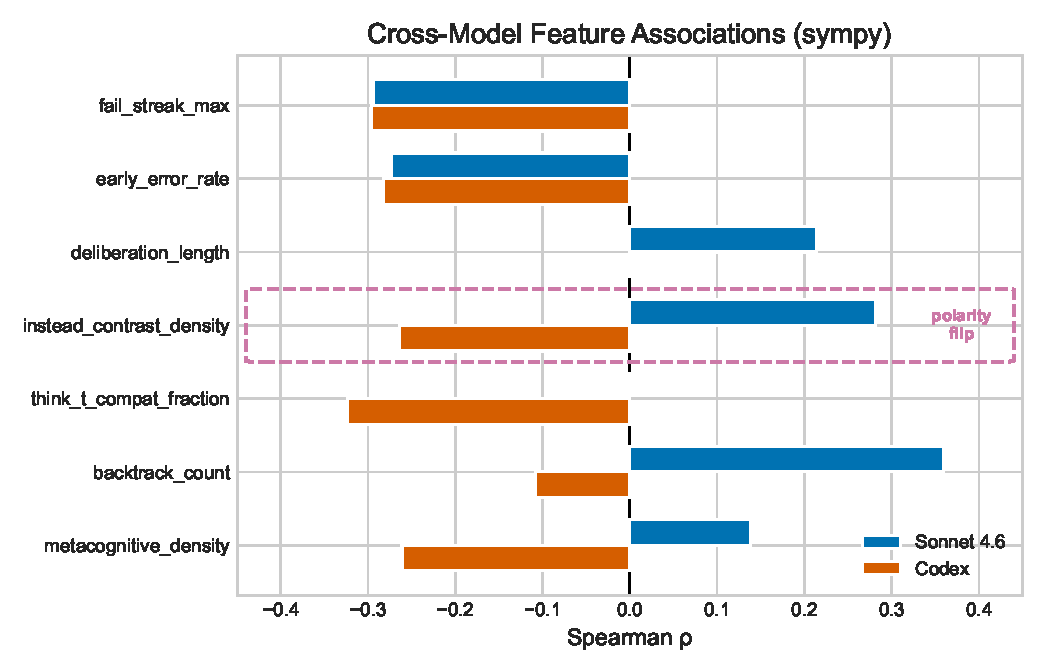
\includegraphics[width=0.85\textwidth]{figures/fig3_cross_model.pdf}
\caption{Cross-model feature comparison. Spearman $\rho$ values for surviving features in Sonnet (horizontal axis) vs.\ Codex (vertical axis), both within sympy. Gold-tier features (error streak, early error rate) cluster in the lower-left quadrant (negative association in both models). The confirmed polarity flip on contrastive density appears as a point in the upper-right/lower-left off-diagonal. Model-specific features cluster along the axes.}
\label{fig:crossmodel}
\end{figure}


% ============================================================
\section{Discussion}
\label{sec:discussion}

What do these surviving features reveal about the nature of behavioral signal in agent reasoning, and what do they imply for practical monitoring systems?

\subsection{Implications for Behavioral Monitoring Design}

The strongest signals associated with agent task success live in layers invisible to a human reviewing the agent's output.
Three categories of signal are systematically hidden.

First, the most diagnostic behavioral features reside in internal reasoning, not in agent messages.
Sonnet's extended thinking blocks contain roughly 10$\times$ more text per run than its polished messages (approximately 11,000 vs.\ 1,200 characters).
Within those thinking blocks, tentative language density shows a significant negative association with success ($\rho = -0.346$, $p = 0.003$; Table~\ref{tab:layer}), while the same feature extracted from messages does not reach significance ($\rho = -0.204$, $p = 0.083$).
A human reading only the agent's messages---which is the default experience for users of chat-based coding assistants---would miss the strongest individual linguistic signal in our dataset.
The diagnostic precision feature, which measures the density of code-specific references (function names, file paths, line numbers) per thousand characters of internal reasoning, distinguishes high-success from low-success configurations at 4--16$\times$ ratios (Table~\ref{tab:interaction}).
None of this is visible in the message stream.

Second, the strongest practical association is not a single feature but the interaction reported in Table~\ref{tab:interaction}.
The combination of high deliberation length and high diagnostic precision yields a 73\% pass rate, while either feature alone yields 23--32\%.
The interaction bonus of $+0.56$ far exceeds any main effect.
A monitoring system that tracks individual features in isolation would, if these associations hold out of sample, miss this nonlinear structure.
An agent that reasons at length but imprecisely (23\% pass) actually performs worse than one that barely reasons at all (38\% pass).
Length without precision is a marker of unproductive rumination, not careful analysis---a finding that contradicts the naive intuition that ``more thinking is better.''
This is precisely the kind of finding that requires simultaneous multi-feature monitoring rather than independent threshold checks.

Third, the polarity of linguistic features is model-specific in ways that would mislead a human observer applying intuition from one model to another.
The confirmed polarity flip on contrastive marker density (Table~\ref{tab:polarity}) means that words like ``however,'' ``but,'' and ``instead'' are associated with success in Sonnet and failure in Codex within the same repository.
A human who learned to read Sonnet's contrastive language as a positive sign would misinterpret the identical pattern in Codex output.

Together, these three categories---hidden layers, hidden interactions, hidden polarities---define the scope of what behavioral exhaust mining can add beyond human review.
The information exists in the traces that agents already produce.
The challenge is extraction and interpretation, not collection.

\subsection{Implications for Gating}

The findings, if they survive intervention testing, have four implications for the design of behavioral gates.

\textbf{Gates would need to be model-specific.}
The confirmed polarity flip, combined with entirely different surviving feature sets for each model, rules out universal feature thresholds.
No feature survives in both models: Sonnet retains \feat{deliberation\_length} and \feat{first\_edit\_position}; Codex retains \feat{think\_t\_compat\_fraction} and \feat{instead\_contrast\_density}.
A gate calibrated on Sonnet's behavioral exhaust would misclassify Codex runs on at least one feature, and vice versa.
This model-specificity also implies that any deployed gate would require recalibration when the underlying model is updated---a practical constraint that limits the utility of behavioral gating in production systems where model versions change frequently.

\textbf{Gates should focus on the early trajectory.}
As shown in Table~\ref{tab:degradation}, feature-outcome associations are significant in the early (0--33\%) and middle (33--67\%) segments but collapse to near-zero in the late segment (67--100\%).
Early error rate, one of only two cross-model features, is by definition an early-trajectory measurement.
By the late trajectory, the agent has either converged on a solution or committed to a failing approach, and reasoning features no longer differentiate the two.
This temporal structure is consistent with the general finding that failing runs produce 35\% more tool calls than passing runs: the late trajectory of a failing run is dominated by increasingly unproductive iterations that look qualitatively similar regardless of the eventual outcome.

\textbf{Nonlinear gates should outperform linear ones.}
The deliberation-by-precision interaction (Table~\ref{tab:interaction}) suggests that a gate checking whether both conditions are met simultaneously would substantially outperform a gate checking either condition alone.
In the quadrant analysis, the high-both cell achieves 73\% pass, while the best single-feature cell achieves only 32\%.
A linear combination of the two features cannot capture this interaction without an explicit interaction term.
Whether this advantage survives out-of-sample evaluation is unknown---the quadrant analysis operates on approximately 22 runs per cell---but the magnitude of the interaction bonus ($+0.56$) motivates the more complex gate design.

\textbf{Gates would need to specify which layer to extract from.}
The thinking/message crossover (Tables~\ref{tab:actually}--\ref{tab:layer}) means that a feature extraction pipeline must choose whether to read internal reasoning or agent messages.
Conflating the two layers would cancel real signals: \feat{tentative\_density} in thinking blocks is associated with failure (permutation $p = 0.0012$), while in messages the same feature does not reach significance.
A pipeline that pools all text would observe a diluted or null effect.
This is a practical requirement: the parser bug that caused our pipeline to read messages instead of thinking blocks masked an entire signal layer.

\subsection{The Polarity Flip in Context}

The confirmed polarity flip on \feat{instead\_contrast\_density} illustrates why model-specific calibration is mandatory, not merely advisable.
The same surface form---contrastive language---serves different cognitive functions in different architectures: diagnostic narrowing in Sonnet versus strategy abandonment in Codex (Section~\ref{sec:polarity}).
As noted in Section~\ref{sec:polarity}, this diagnostic-vs-strategic interpretation is post-hoc and based on qualitative inspection of a small number of examples; it should be treated as a hypothesis for future systematic coding analysis.
Any study that pools linguistic features across models without checking for polarity consistency will wash out real signals.
In our combined-model analysis, contrastive density has no significant association with success precisely because the positive Sonnet signal and the negative Codex signal cancel.

A confound must be acknowledged.
Sonnet and Codex produce internal reasoning in architecturally different formats.
Sonnet's extended thinking blocks cover 100\% of runs but only 28\% of individual tool calls have per-call reasoning annotations, while Codex's reasoning items cover 100\% of runs and 60.1\% of calls.
The per-call coverage difference means that the linguistic features extracted from per-call reasoning text are computed over different samples of the agent's behavior in each model.
It is possible that the polarity flip partly reflects this sampling difference rather than a genuine difference in how the models use contrastive language.
Future work should examine whether the flip persists when features are extracted only from the thinking-block layer, where coverage is 100\% for both models.

Two additional features---\feat{backtrack\_count} and \feat{metacognitive\_density}---show suggestive directional reversals (opposite signs across models, but only one side reaches significance; Table~\ref{tab:polarity}).
These are hypotheses for future testing, not confirmed findings.
If they replicate, they would strengthen the case that model-specific calibration is a fundamental requirement for behavioral exhaust mining.

\subsection{Relationship to the Faithfulness Literature}

The thinking/message crossover is consistent with \citet{chen2025unfaithful}'s finding that chain-of-thought content is unfaithful approximately 75\% of the time.
Our data adds a nuance: even when internal reasoning diverges from what the agent expresses publicly, the \emph{structure} of both layers still carries signal associated with task outcomes.
Unfaithfulness, in this framing, is not the absence of signal but the presence of \emph{different} signal in different layers.

The ``actually'' polarity reversal (Table~\ref{tab:actually}) is illustrative but must be interpreted with caution: the thinking-block ``actually'' density does not survive the within-repo permutation test ($p = 0.436$), while \feat{tentative\_density} in thinking blocks does ($p = 0.0012$).
The permutation test validates the layer difference for tentative language but not for the ``actually'' token specifically.
The crossover finding is therefore better characterized as: internal doubt markers in thinking blocks carry genuine signal, while the specific lexical item ``actually'' shows an illustrative but non-robust reversal.
In agent messages, ``actually'' marks performative self-correction---a display of metacognitive competence for the user, which is positively associated with success ($\rho = +0.494$, 95\% CI [$+0.376$, $+0.596$]).
A faithfulness-focused analysis that asked ``does the thinking match the message?'' would correctly flag the mismatch but would miss the fact that both layers are independently useful.

This suggests a reframing of the faithfulness question for agent monitoring: rather than asking whether the agent's public reasoning faithfully represents its private reasoning (it does not), we should ask what each layer reveals about the agent's state.
Internal reasoning reveals genuine uncertainty; expressed reasoning reveals the agent's model of what successful problem-solving looks like.
Both are useful for reliability estimation, provided they are extracted and interpreted separately.

\citet{chen2025unfaithful} also observed that unfaithful chains of thought are systematically longer than faithful ones.
Our finding that \feat{deliberation\_length} is positively associated with success in Sonnet may appear to contradict this, but the two results measure different things.
Chen et al.\ measure total CoT length in a QA setting where longer reasoning often reflects unnecessary elaboration.
We measure per-call reasoning length in an agent setting where longer reasoning per action reflects more thorough consideration before each step.
The per-call normalization is critical: total reasoning length correlates with total tool calls (which correlates with failure), but per-call reasoning length is associated with success.

\subsection{Implications for Agent Safety Research}

The central practical finding is that behavioral exhaust carries signal associated with task outcomes, extractable at zero additional API cost.
For agent safety research, this has several implications.

First, behavioral features could serve as runtime monitoring signals.
The structural features (error streaks, early error rate) are model-agnostic and could be deployed as lightweight anomaly detectors without model-specific calibration.
When an agent accumulates three or more consecutive errors, or when its early-trajectory error rate exceeds a threshold, the system could flag the run for human review or trigger an intervention.
These features survived all our statistical tests and showed consistent direction across both models.

Second, the model-specificity of linguistic features means that any behavioral monitoring system calibrated on one model version will require recalibration when the model is updated.
This is a maintenance cost that production systems must budget for.
The magnitude of recalibration is not trivial: a feature that is the strongest Sonnet-specific signal (\feat{deliberation\_length}) is not significant in Codex, and a feature that flips polarity entirely (\feat{instead\_contrast\_density}) would produce actively wrong classifications if the calibration from one model were applied to another.
The only features that appear to transfer are structural ones that do not depend on the content of reasoning text.

Third, all findings are associational, not causal.
We have not demonstrated that a gate built on these features would improve outcomes, nor have we computed the operating characteristics (sensitivity, specificity, false positive rate) that would be required for deployment.
The distance between ``this feature is associated with success'' and ``this feature can be used to improve agent reliability'' is substantial and must be bridged by intervention testing.
Anthropic's own methodology for model evaluations \citep{anthropic2025evaluations} emphasizes paired comparison designs and clustered standard errors for exactly this kind of within-subject testing.

\citet{srikumar2025prioritizing} argue for prioritizing real-time failure detection in deployed AI agents; the behavioral features identified here are candidates for the kind of runtime monitoring they envision, though our work demonstrates associations rather than a deployable detection system.

\begin{figure*}[t]
\centering
\resizebox{\textwidth}{!}{% TikZ Evidence Hierarchy Diagram
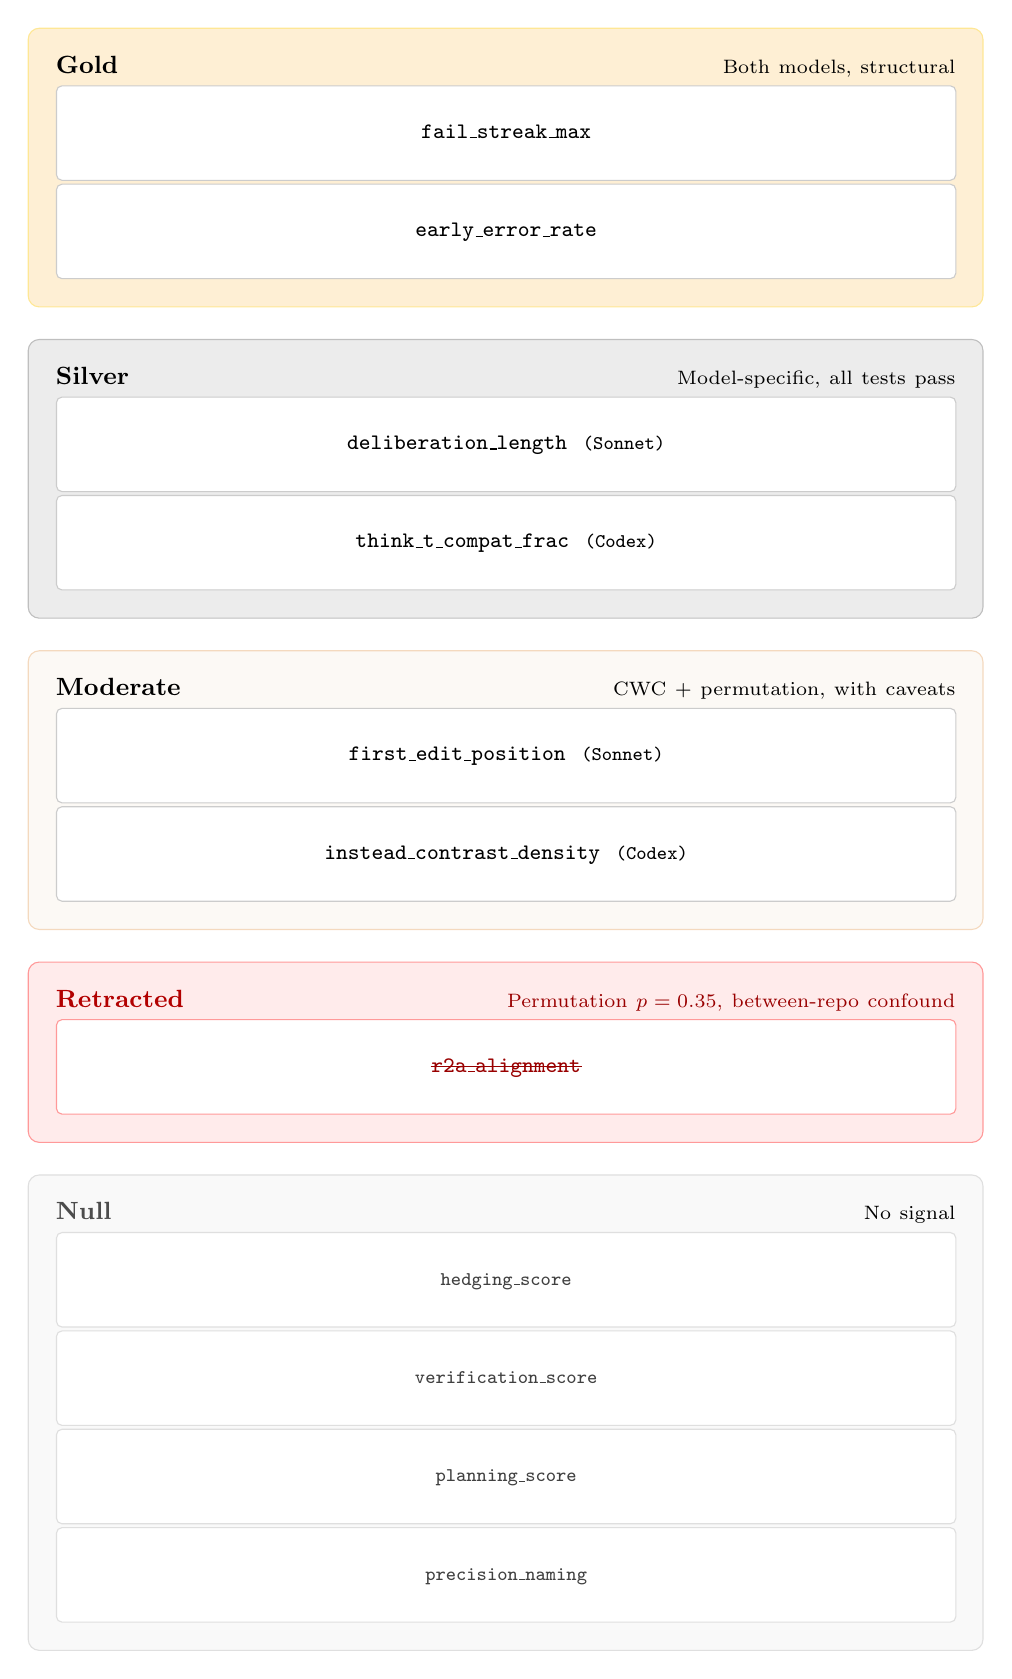
\begin{tikzpicture}[
    >=Stealth,
    node distance=0.4cm,
    every node/.style={font=\small},
    tier/.style={draw, rounded corners=4pt, minimum width=\textwidth, minimum height=1.2cm, text width=\textwidth-20pt, align=left, font=\small, inner sep=10pt},
    featbox/.style={font=\footnotesize\ttfamily, fill=white, draw=gray!40, rounded corners=2pt, inner sep=3pt},
]

% ---- Gold ----
\node[tier, fill=yellow!25!orange!15, draw=yellow!60!orange!40] (gold) {%
  \textbf{Gold} \hfill {\scriptsize Both models, structural}\\[2pt]
  \tikz[baseline=(a.base)]{\node[featbox](a){\strut fail\_streak\_max};}
  \hspace{6pt}
  \tikz[baseline=(b.base)]{\node[featbox](b){\strut early\_error\_rate};}
};

% ---- Silver ----
\node[tier, fill=gray!15, draw=gray!50, below=of gold] (silver) {%
  \textbf{Silver} \hfill {\scriptsize Model-specific, all tests pass}\\[2pt]
  \tikz[baseline=(a.base)]{\node[featbox](a){\strut deliberation\_length\, \scriptsize(Sonnet)};}
  \hspace{6pt}
  \tikz[baseline=(b.base)]{\node[featbox](b){\strut think\_t\_compat\_frac\, \scriptsize(Codex)};}
};

% ---- Moderate ----
\node[tier, fill=orange!10!brown!5, draw=orange!40!brown!30, below=of silver] (moderate) {%
  \textbf{Moderate} \hfill {\scriptsize CWC + permutation, with caveats}\\[2pt]
  \tikz[baseline=(a.base)]{\node[featbox](a){\strut first\_edit\_position\, \scriptsize(Sonnet)};}
  \hspace{6pt}
  \tikz[baseline=(b.base)]{\node[featbox](b){\strut instead\_contrast\_density\, \scriptsize(Codex)};}
};

% ---- Retracted ----
\node[tier, fill=red!8, draw=red!40, below=of moderate] (retracted) {%
  \textbf{\color{red!70!black}Retracted} \hfill {\scriptsize\color{red!60!black} Permutation $p = 0.35$, between-repo confound}\\[2pt]
  \tikz[baseline=(a.base)]{\node[featbox, draw=red!40, text=red!60!black](a){\strut\sout{r2a\_alignment}};}
};

% ---- Null ----
\node[tier, fill=gray!5, draw=gray!25, below=of retracted] (null) {%
  \textbf{\color{gray!60!black}Null} \hfill {\scriptsize No signal}\\[2pt]
  \tikz[baseline=(a.base)]{\node[featbox, draw=gray!25, text=gray!50!black](a){\strut\scriptsize hedging\_score};}
  \hspace{4pt}
  \tikz[baseline=(b.base)]{\node[featbox, draw=gray!25, text=gray!50!black](b){\strut\scriptsize verification\_score};}
  \hspace{4pt}
  \tikz[baseline=(c.base)]{\node[featbox, draw=gray!25, text=gray!50!black](c){\strut\scriptsize planning\_score};}
  \hspace{4pt}
  \tikz[baseline=(d.base)]{\node[featbox, draw=gray!25, text=gray!50!black](d){\strut\scriptsize precision\_naming};}
};

\end{tikzpicture}
}
\caption{Evidence hierarchy for behavioral features. Features are arranged by the strength of statistical evidence supporting their association with task success: Gold (both models, structural), Silver (model-specific, all tests passed), Moderate (CWC and permutation but with caveats), Retracted (failed permutation), and Null (no signal). Only two features---both structural---achieve Gold status; no linguistic feature transfers across models.}
\label{fig:hierarchy}
\end{figure*}


% ============================================================
\section{Limitations}
\label{sec:limitations}

We identify eleven limitations, grouped by their impact on interpretation.

\textbf{Correlational design.}
No causal intervention was performed.
The association between a behavioral feature and task success may be confounded by task difficulty: easier tasks may simultaneously elicit better reasoning structure and produce more successful outcomes.
The retraction of \rtalign{} (Section~\ref{sec:retraction}) illustrates how correlational findings can mislead.

\textbf{Modest predictive performance.}
The nested LOO-CV AUC of 0.569 (Sonnet, marginal) and 0.634 (Codex, significant) confirms that the behavioral features carry real out-of-sample signal but are far from sufficient for practical deployment.
The gap between observational association and deployable prediction remains the central open question.

\textbf{No prospective evaluation.}
Although the LOO-CV provides out-of-sample AUC estimates, there is no prospective intervention test, no calibration analysis, and no evaluation under deployment conditions.
The interaction effect (73\% pass in the high-deliberation, high-precision quadrant) is an observational association, not a validated decision rule.

\textbf{Model-specificity.}
Linguistic features do not transfer across models.
The polarity flip and the disjoint surviving feature sets mean our findings are specific to these two model versions.
Only the two structural features showed consistent direction across both architectures.

\textbf{Narrow domain.}
All tasks are drawn from SWE-bench Lite, a corpus of Python bug-fix tasks.
Whether similar features would be informative for other agent tasks---web browsing, data analysis, multi-step planning---is unknown.

\textbf{Sample size per cell.}
The within-repo analyses operate on cells of $n = 44$ to $n = 87$.
The interaction analysis uses quadrant splits with approximately 22 runs per cell.
These sizes provide adequate power for medium-to-large effects but may miss smaller associations.

\textbf{Thinking block format differences.}
Per-call reasoning text coverage differs substantially (28\% for Sonnet vs.\ 60\% for Codex).
Cross-model comparisons of linguistic features extracted from these different formats must be interpreted with caution.

\textbf{Codex convergence.}
Codex's sympy pass rate improved by 10.3 percentage points from early to late runs.
While within one standard deviation of random variation for the sample size, this trend could reflect infrastructure stabilization or task-ordering effects.
If the improvement is genuine, early Codex runs are biased downward, which would affect the Codex-specific feature associations reported for sympy.

\textbf{Within-repo permutation scope.}
The permutation test controls for between-repo confounds but not within-repo task difficulty variation.
A within-task permutation test---shuffling labels among replicates of the same task---is the stronger design but requires sufficient mixed-outcome tasks.
Our within-task analysis is limited to 7 Sonnet tasks (35 runs) and 5 Codex tasks (18 runs) with mixed outcomes.
Given the small sample (7 tasks, 35 runs), the within-task result should be treated as suggestive rather than confirmatory.
No task has mixed outcomes in both models simultaneously, precluding cross-model within-task permutation.

\textbf{Unmatched task sets.}
Five tasks were run on Sonnet but not Codex.
All cross-model comparisons use the 70 shared tasks, but the five Sonnet-only tasks could bias Sonnet-specific feature estimates if those tasks have unusual behavioral profiles.

\textbf{Single labeler.}
All correctness labels were assigned by a single researcher using a blinded dual-pass protocol (independent validation via test replay, not agent self-report).
While the validation is automated and deterministic once the test suite is specified, the decision to classify ambiguous cases (e.g., partial test passage, infrastructure failures) reflects one person's judgment.
Four runs were excluded as unrecoverable.
Inter-rater reliability was not assessed.

\textbf{Non-random task selection.}
Tasks were selected to produce a blended pass rate near 50\%, providing balanced classes for correlation analysis.
This convenience sampling may not represent the true distribution of SWE-bench difficulty, and the feature associations we observe could differ on tasks with more extreme pass rates.


% ============================================================
\section{Conclusion}
\label{sec:conclusion}

We studied whether structural properties of agent reasoning traces are associated with task success in code repair.
Across 373 validated runs from two models on 75 SWE-bench Lite tasks, we extracted 24 primary behavioral features at zero API cost and subjected them to within-repo correlation, Fisher-combined CWC decomposition, and within-repo permutation testing.

Three findings emerged.
First, behavioral exhaust carries signal, but that signal is model-specific.
Only two structural features---consecutive error streaks and early error rate---show consistent associations with failure across both models.
All surviving linguistic features are model-specific, and one (contrastive marker density) flips polarity entirely (Section~\ref{sec:polarity}).
Second, the strongest observational association is not a single feature but an interaction: in Sonnet, the combination of high deliberation length and high diagnostic precision yields a 73\% pass rate, while either feature alone yields 23--32\% (Table~\ref{tab:interaction}).
This nonlinear structure would be invisible to monitoring systems that track features independently.
Third, internal reasoning and agent messages carry structurally different information: tentative language in thinking blocks is significantly associated with failure (permutation $p = 0.0012$), while expressed correction in messages is associated with success (Section~\ref{sec:crossover}).
The specific ``actually'' reversal, though illustrative, does not survive permutation testing ($p = 0.436$).

A leave-one-task-out cross-validation with nested feature selection yields AUC = 0.569 for Sonnet ($p = 0.064$, marginal) and 0.634 for Codex ($p < 0.001$, significant)---genuine out-of-sample signal for structural features that bridges the gap between the observational associations reported here and the prospective intervention testing planned for Phase~1.
These findings are associational.
We have not demonstrated that a gate built on these features would improve agent reliability.
The natural next step is intervention testing: gating agent tool calls based on the model-specific features identified here and measuring whether gated runs outperform ungated runs using paired within-subject designs.
The post-hoc gate simulation (Appendix~\ref{app:gate}) provides preliminary estimates of gate operating characteristics and identifies design flaws---particularly the contamination of the gate by the retracted alignment feature---that must be corrected before intervention testing.
Anthropic's published methodology for model evaluations---clustered standard errors, pass$^k$ metrics, and pre-registered power analysis---provides the statistical framework for that test.

The contribution of this work is establishing that the behavioral exhaust these two models produce on Python code repair tasks---reasoning text structure, tool-call error patterns, thinking block content---carries model-specific signal associated with task outcomes.
This signal is free to extract, requires no prompt modification, and opens a measurement dimension complementary to existing approaches based on verbalized confidence or external critics.
Whether that measurement dimension can be converted into a practical reliability improvement remains an open question.


% ============================================================
\appendix

\section{Post-Hoc Gate Simulation}
\label{app:gate}

\textbf{Note:} The alignment check component of this gate is based on \rtalign{}, which was retracted (Section~\ref{sec:retraction}).
The simulation results should be interpreted accordingly.

To bridge the observational findings and the planned intervention experiment, we apply the introspective behavioral gate post-hoc to all 181 validated Sonnet runs.
This simulation measures what the gate \emph{would have done} on the exact trajectories already collected, providing precision and recall estimates without new data collection.

\subsection{Gate Design}

The introspective gate evaluates each Edit/Write tool call on two criteria derived from passing runs:

\begin{enumerate}[leftmargin=*]
\item \textbf{Alignment check:} Does the reasoning text preceding the edit mention the target file by name or path? (Binary; threshold = 0.5)
\item \textbf{Deliberation check:} Is the reasoning text at least 117 characters? (Median per-call length from passing runs)
\end{enumerate}

If either check fails, the call is flagged as ``blocked.''
Ground truth is operationalized at the run level: a blocked call in a failing run is a true positive.

The gate applies only to Sonnet.
Codex never uses Edit or Write tools---it performs all file modifications through Bash commands.
This architectural difference means the introspective gate as designed is inherently model-specific, consistent with the broader finding that behavioral features do not transfer across models.

\subsection{Results}

We evaluate two timing conditions: A1 (gate applied to the first third of the trajectory only) and B1 (gate applied to all calls).

\begin{table}[t]
\centering
\caption{Post-hoc gate simulation results.}
\label{tab:gate}
\small
\begin{tabular}{lccccc}
\toprule
\textbf{Condition} & \textbf{Calls Eval.} & \textbf{Blocked} & \textbf{Block Rate} & \textbf{Precision} & \textbf{Recall} \\
\midrule
A1 (early)  & 553 & 180 & 32.5\% & 0.628 & 0.388 \\
B1 (always) & 553 & 514 & 92.9\% & 0.545 & 0.962 \\
\bottomrule
\end{tabular}
\end{table}

B1 is impractical: it blocks 93\% of all edits.
A1 is more selective, blocking roughly one-third of early-trajectory edits with 63\% precision---above the 50.8\% base failure rate but far from deployable.

\begin{table}[t]
\centering
\caption{Gate precision by repository.}
\label{tab:gaterepo}
\small
\begin{tabular}{lcccc}
\toprule
\textbf{Repository} & \textbf{Edit/Write Calls} & \textbf{Blocked} & \textbf{Precision} & \textbf{Base Fail Rate} \\
\midrule
sympy      & 249 & 63 & 0.762 & 58.6\% \\
pytest-dev & 118 & 40 & 0.900 & 71.4\% \\
django     & 138 & 50 & 0.200 & 15.9\% \\
\bottomrule
\end{tabular}
\end{table}

Gate precision varies widely by repository.
On sympy (balanced difficulty), A1 achieves 76\% precision.
On django (84\% pass rate), precision drops to 20\%: the gate flags many edits in runs that ultimately succeed.

\subsection{Interpretation}

The simulation yields three findings relevant to intervention design.

First, \textbf{the gate as designed is not deployable}.
Precision of 63\% overall, with 20\% on the highest-volume repository, would produce unacceptable false-positive rates.

Second, \textbf{repository base rate dominates gate precision}.
Any practical gate must condition on difficulty estimates or repository-specific thresholds.

Third, \textbf{the retracted feature contaminates the gate}.
The alignment check---the gate's primary blocking mechanism---is derived from \rtalign{}, whose observational association was inflated by between-repo confounding (Section~\ref{sec:retraction}).
A revised gate should replace the alignment check with \feat{deliberation\_length} (perm $p = 0.0004$) and the deliberation $\times$ diagnostic precision interaction, which survived all statistical tests.

These findings motivate a revised gate design for intervention testing---one that uses the features which survived the full statistical battery rather than those available at the time the gate was initially designed.


\section{Complete Feature Definitions}
\label{app:features}

\begin{table}[t]
\centering
\caption{Complete feature definitions (24 primary features + 3 supplementary). Supplementary features marked with *.}
\label{tab:features}
\small
\begin{adjustbox}{max width=\textwidth}
\begin{tabular}{p{4cm}ccp{6.5cm}}
\toprule
\textbf{Feature} & \textbf{Tier} & \textbf{Source} & \textbf{Definition} \\
\midrule
\feat{fail\_streak\_max}       & 0 & tool\_calls & Maximum consecutive error results in the tool-call sequence \\
\feat{early\_error\_rate}      & 0 & tool\_calls & Fraction of calls returning errors in the first third of the trajectory \\
\feat{first\_edit\_position}   & 0 & tool\_calls & Normalized position (0--1) of the first Edit or Write call \\
\feat{unique\_files\_touched}  & 0 & tool\_calls & Count of distinct files edited \\
\feat{edit\_churn\_rate}       & 0 & tool\_calls & Total edit operations divided by unique files touched \\
\feat{test\_run\_count}        & 0 & tool\_calls & Count of Bash calls whose command contains ``test'' \\
\feat{n\_calls}                & 0 & tool\_calls & Total state-modifying tool calls (control variable) \\
\feat{hedging\_score}          & 1 & reasoning & Density of Hyland hedge terms per token \\
\feat{deliberation\_length}    & 1 & reasoning & Mean characters per reasoning block across calls \\
\feat{backtrack\_count}        & 1 & reasoning & Density of backtrack markers per token \\
\feat{verification\_score}     & 1 & reasoning & Density of verification phrases per token \\
\feat{planning\_score}         & 1 & reasoning & Density of planning phrases per token \\
\feat{metacognitive\_density}  & 2 & reasoning & Density of self-correction markers per token \\
\feat{tentative\_density}      & 2 & reasoning & Density of tentative language per token \\
\feat{insight\_density}        & 2 & reasoning & Density of insight phrases per token \\
\feat{instead\_contrast\_density} & 2 & reasoning & Density of contrastive markers per token \\
\feat{self\_directive\_density} & 2 & reasoning & Density of self-directive language per token \\
\feat{precision\_naming\_score} & 2 & reasoning & Density of backtick-delimited identifiers per token \\
\rtalign{} & X & reasoning + tools & Binary: does reasoning preceding an edit name the target file? Mean across calls \\
\feat{think\_diag\_precision} & CWC & thinking & Density of code-specific references per 1K chars \\
\feat{think\_reason\_clarity} & CWC & thinking & Diagnostic precision minus confusion score \\
\feat{think\_t\_func\_refs}   & CWC & thinking & Density of function/method references per 1K chars \\
\feat{think\_t\_compat\_frac} & CWC & thinking & Fraction of sentences discussing compatibility/environment \\
\feat{think\_t\_pivots}       & CWC & thinking & Density of strategy pivot markers per 1K chars \\
\midrule
\feat{recovery\_rate}*         & 0 & tool\_calls & Fraction of error calls followed by a successful call \\
\feat{fail\_then\_switch\_rate}* & 0 & tool\_calls & Fraction of error calls followed by a different tool \\
\feat{causal\_density}*        & 2 & reasoning & Density of causal markers per 1000 chars \\
\bottomrule
\end{tabular}
\end{adjustbox}
\end{table}


% ============================================================
\bibliography{references}

\end{document}
